\documentclass{article}
\usepackage{graphicx}
\usepackage{wrapfig}
\usepackage{xcolor}
\usepackage{hyperref}
\usepackage{multicol}

\setlength{\textheight}{25cm}
\setlength{\textwidth}{152mm}
\setlength{\topmargin}{-2.5cm}
\setlength{\evensidemargin}{12mm}
\setlength{\oddsidemargin}{6mm}
\definecolor{my_col}{RGB}{0,150,150}
\pagenumbering{gobble}

\sffamily

\begin{document}

\begin{center}
	\textit{\Huge Curriculum Vitae}   
	\vspace*{1cm}
\end{center}

\begin{wrapfigure}{r}{0.25\textwidth} 
	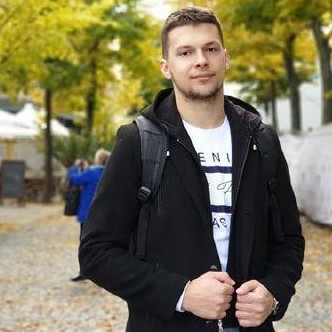
\includegraphics[width=0.25\textwidth]{my_pic.jpeg}
\end{wrapfigure}

\color{my_col}
\textbf{\large PERSONAL INFORMATION}\\
\noindent\rule{10cm}{1.5pt}\color{black}\\ \\
Name:  \textbf{\emph{Predrag MITIC}} \\
Address: \emph{Antifasiticke borbe, Belgrade, Serbia }\\
Tel: 	(+381) 61 18 56 816 \\
E-mail1:	\textit{predrag98mitic@gmail.com} \\ 
E-mail2:	\textit{pmitic@hotmail.com} \\ 
Web:	\url{www.alas.matf.bg.ac.rs/~mi17116} \\
Github:	\url{www.github.com/PredragMitic} \\ 
LinkedIn: \url{www.linkedin.com/in/predrag-mitic-353019188}\\
Date of Birth: September 1, 1998 \\ 

\color{my_col}
\textbf{\large PROFILE}\\
\noindent\rule{15.4cm}{1.6pt}\color{black}\\ 
Ambitious and highly motivated Game Developer, with 3 years experience in developing Web Games for gambling industry. Skilled in games architecture, optimizing game performances and game quality improvement in general. Proven ability to manage project development and timelines. 
Team player, quick learner, open to new ideas and experiences.\\ \\
\textit{\textbf{English level: } B2}\\

\color{my_col}
\textbf{\large PROGRAMMING LANGUAGES}\\
\noindent\rule{15.4cm}{1.6pt}\color{black}
\normalsize
\begin{itemize}
	\item\textbf{Good knowledge: 	} Typescript, Python3, C/CPP
	\item\textbf{Some experience:	} Haskell, Scala, R, Java
	\item\textbf{Frameworks used:} PixiJS, AnimeJS, QT5\\
\end{itemize}
  
\color{my_col}
\textbf{\large COMPUTER SKILLS}\\
\noindent\rule{15.4cm}{1.6pt}\color{black}
\normalsize
   \begin{multicols}{2}
  	\begin{itemize}
  		\item\textbf{OS: 	} Windows, GNU/Linux
  		\item\textbf{Documents:} MS Office, Libre Office, \LaTeX
  		\item\textbf{Markup Language: } HTML, CSS, Markdown\\
  		\item\textbf{Image editing: } Gimp
  		\item\textbf{Editors :} Visual Studio (Code), Vim, JetBrains(CLion, PyCharm, Idea), Jupyter Notebook, Atom\\
 
  	\end{itemize}
  \end{multicols}

\color{my_col}
\textbf{\large EMPLOYMENTS AND TRAINING}\\
\noindent\rule{15.4cm}{1.6pt}\color{black}
\begin{description}
	\item[ 2019] - RT-RK Summer School \\
	\textit{Modern Improvements in C++}\\
	\item[ 2020 - 2021] - Finbet - Full Stack Game Development Internship\\
	\textit{Worked on online multiplayer game development. Developed both frontend and backend app sides, so communication between this two side was implemented on socket systems. Client application is developed in Javascript within following frameworks PixiJS and AnimeJS. Backend side was a node application.}\\
	\item[ 2021 - present ] - Finbet - Frontend Game Developer \\
	\textit{Joined a team that prioritizes a variety of projects, with games taking the top spot. We have been working on developing in-house engine and editor that made the process easier and better. PixiJS is the main framework, around which we made the engine. Editor is made in HTML/CSS without any frameworks.}\\
\end{description}

\color{my_col}
\textbf{\large FACULTY PROJECTS}\\
\noindent\rule{15.4cm}{1.6pt}\color{black}
\begin{description}
	\item[ C/OpenGL] - Shoot Training\\ 
	Game made in C program language and OpenGl(Open Graphics Library)
	\item[ Python3/Pygame] - Star Wars Space Battle\\ 
	Game like Galaga made in pygame with Star Wars motives.\\
	This game is built by team Jedi-MATF for course project.
\end{description}
My projects with other details can be seen on my GitHub profile \\

\color{my_col}
\textbf{\large SCIENTIFIC INTERESTS}\\
\noindent\rule{15.4cm}{1.6pt}\color{black}\\\\
- Algorithm and Data Structures\\
- Computer vision \\
- Computer Graphics and Game Development\\
- Mobile App Development\\

\color{my_col}
\textbf{\large EDUCATION}\\
\noindent\rule{15.4cm}{1.6pt}\color{black}
\begin{description}
    \item[ 2017-present : Bachelor of Informatics ]\hfill \\
    \textbf{\textit{Faculty of Mathematics, University of Belgrade}}\\
\end{description}

\begin{description}
    \item[ 2013-2017 : Mechatronics Technician]\hfill \\
    \textbf{\textit{High School of Technology, Leskovac}}\\
    \normalsize \\
  
\end{description}
\color{my_col}
\textbf{\large ACHIEVEMENTS}\\
\noindent\rule{15.4cm}{1.6pt}\color{black}
\normalsize

\begin{description}
	\item[ 2016] - Fourth place in 3D Computer Graphics (Autodesk Inventor)\\
	National Competition
	\item[ 2016] - Second place in Electronics\\
	National Competition
	\item[ 2015] - First place in 2D Computer Graphics (Autodesk AutoCAD)\\
	Regional Competition
	\item[ 2014] - First place in 2D Computer Graphics (Autodesk AutoCAD)\\
	National Competition
\end{description}

\color{my_col}
\textbf{\large FREE TIME }\\
\noindent\rule{15.4cm}{1.6pt}\color{black}\\\\
- Travel and Languages\\
- Sport (Basketball, Swimming, Bodybuilding) \\
- Art (Movies, Music, Books)\\
- Geography\\

\color{my_col}\noindent\rule{15.4cm}{1.6pt}\color{black}
\begin{flushright}
	\small Belgrade, May 2024.
\end{flushright}

\end{document}
